\subsection{Polygonal Linkages}
\begin{figure}[h]
\begin{center}

\includegraphics[scale=1]{graphics/hingeOnThreeDistinctPolygons.pdf}
\end{center} 
\caption{(a) A polygonal linkage with a non-convex polygon and two hinge points corresponding to 
three polygons.  Note that hinge points correspond to two distinct polygons.(b) Illustrating that 
two hinge points can correspond to the same boundary point of a polygon.}
\label{fig:linkage-1}
\end{figure}
%describe how it is a generalization of Linkages.
Polygonal linkages have some differences to linkages.  Polygonal linkages have a combinatorial 
structure that is graph-like.  A polyonal linkage's combinatorial structure is an ordered pair 
$\left(\HH,\PP \right)$.  Instead of a set of vertices, there is a set of hinges, $\HH$;  instead 
of a set of edges, there is a set of polygons, $\PP$. Formally, a \textit{hinge} $h\in \HH$ 
corresponds to two points on the boundary of two distinct polygons in $\PP$.  Since polygons do not 
exhibit a length property, a polygonal linkage does not have an edge length mapping.  


Polygon linkages are similar to linkages.  They are an ordered pair of sets, with the exception 
that the set of vertices become a set of hinges, $\HH$, and the set of edges become a set of 
polygons, $\PP$.  Formally, a \textit{polygonal linkage} is an ordered pair, $G = (\HH,\PP)$,  
comprises of a set of polygons, $\PP$, and a set of hinge points $\HH$ where each hinge $h \in \HH$ 
corresponds to two points on the boundary of two distinct polygons in $\PP$. Mapping the linkage 
$G$ into the plane is said to be the \textit{embedding}, i.e. $L : \HH \mapsto \bbR^{2}$.  We 
consider a \textit{realization} of a polygonal linkage is range of $L$, i.e. $l(\HH)$.

In figure (\ref{fig:linkage-1}), we illustrate that two hinge points can reside on the same point 
in the plane. Figure (\ref{fig:linkage-1}) and figure (\ref{fig:linkage-3}) are examples of special 
cases that we may run into, but do not want to focus heavily on.  They are presented to the reader 
to facilitate understanding of the definitions of polygonal linkages and linkages respectively.  
Without loss of generality, for this paper, we focus on polygonal linkages that are 
equivalent to simple planar graphs.
%Foigr each hinge point $h \in \HH$, there 
%exists some subset $P \subset \PP$ with 
%at least cardinality of 2 such that for each polygon $p \in P$, $h$ corresponds to some point on 
%the boundary of $p$.  When the polygonal linkage is embedded in the plane, the hinge point is 
%where 
%the polygons of $P$ \it{kiss}.  
% show an example of polygonal linkages
\begin{figure}[h]
\begin{center}
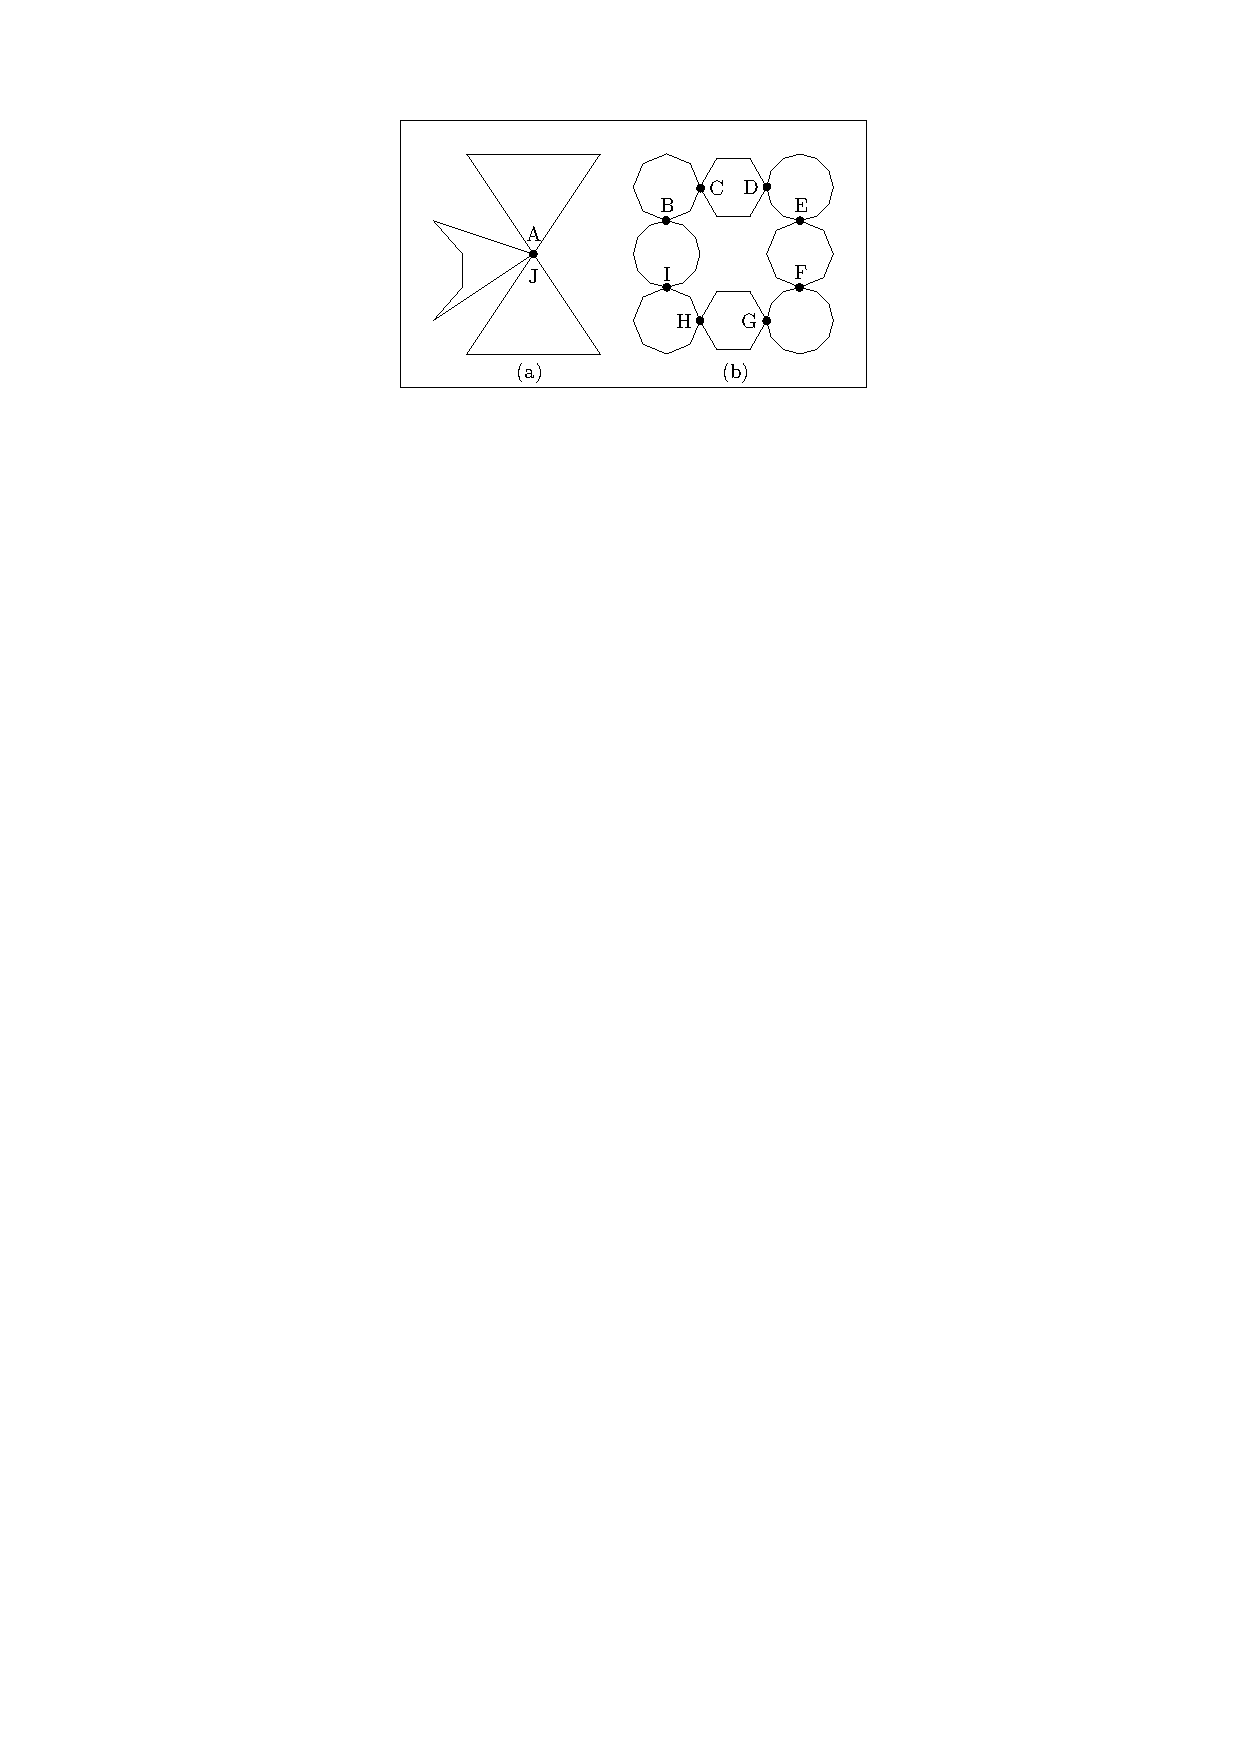
\includegraphics[scale=1]{graphics/PolygonalLinkageExamples.pdf}
\end{center} 
\caption{(a) A polygonal linkage with a non-convex polygon and a hinge point corresponding to three 
polygons.  (b) A polygonal linkage with 8 regular polygons.}
\label{fig:linkage-2}
\end{figure}
For the remainder of this thesis, we'll focus on the polygonal linkages with the following 
restrictions:
\begin{enumerate}
 \item  For each hinge point $h \in \HH$, there exists some subset $P \subset \PP$ with 
exactly cardinality of 2, and
\item every polygon in $\PP$ is convex.
\end{enumerate}
Formally, we define a \it{polygonal linkage} as an ordered pair $L = (\HH,\PP)$ comprising of a 
set of hinges, $\HH$, where each hinge $h\in \HH$ corresponds to two points on the boundary of two 
distinct polygons. A \emph{realization} of a polygonal linkage is an interior-disjoint placement of 
congruent copies of the polygons in $\PP$ such that the points corresponding to each hinge are 
identified (Fig. \ref{fig:1}).